\documentclass[11pt,a4paper]{report}
\usepackage[latin1]{inputenc}
\usepackage[dutch]{babel}
\usepackage{amsmath}
\usepackage{amsfonts}
\usepackage{amssymb}
\usepackage[left=2cm,right=2cm,top=2cm,bottom=2cm]{geometry}
\usepackage{algorithm}
\usepackage{algorithmic}
\usepackage{graphicx}
\author{Niels De Bock \& Mattias De Charleroy \\ 2Ba Informatica}
\date{18 april 2013}
\title{\Huge Practicum: snijdende cirkels \\ \LARGE Toepassingen van de meetkunde in de informatica\\ \normalsize bestemming: Yvette Vanberghen}
\setlength{\parindent}{0pt}
\begin{document}
\maketitle
\newpage

\section*{1. Beschrijving van de algoritmen}
\subsection*{1.1 Algoritme 1}


\begin{algorithm}
\caption{Bereken alle snijpunten van een verzameling cirkels}
\begin{algorithmic}
	\STATE \textbf{Input:}  $cirkels$: Een array met $n$ cirkels
	\STATE $snijpunten$ $\gets \emptyset$
    \FOR{$i = 0 \to n-1$}
       \FOR{$j = i+1 \to n-1$} 
            \STATE  voegToe($snijpunten$, berekenSnijpunten($cirkels[i]$, $cirkels[j]$))
        \ENDFOR
    \ENDFOR
    \RETURN snijpunten
\end{algorithmic}
\end{algorithm}

Dit algoritme zal elk paar cirkels \'e\'en keer met elkaar vergelijken om snijpunten te berekenen, wat neerkomt op $\frac{n(n-1)}{2}$ vergelijkingen. Het berekenen van snijpunten gebeurt op de volgende manier: eerst doen we een snelle check om te bepalen of de twee cirkels daadwerkelijk snijden. Dit kan door de afstand tussen de middelpunten te vergelijken met de som van de stralen. Wanneer deze afstand groter is dan de som van de stralen snijden de cirkels niet. Een cirkel kan echter ook volledig in een andere cirkel liggen. Dit is wanneer de afstand ($d$) tussen de middelpunten kleiner is dan het lengteverschil tussen de stralen ($|r_1-r_2|$). Wanneer twee cirkels gelijk zijn en dus samenvallen, zullen er geen snijpunten berekend worden. Dit is echter een randgeval. Wanneer blijkt dat de cirkels snijden, zullen we de snijpunten berekenen zoals beschreven in sectie 3.

\begin{figure}[h]
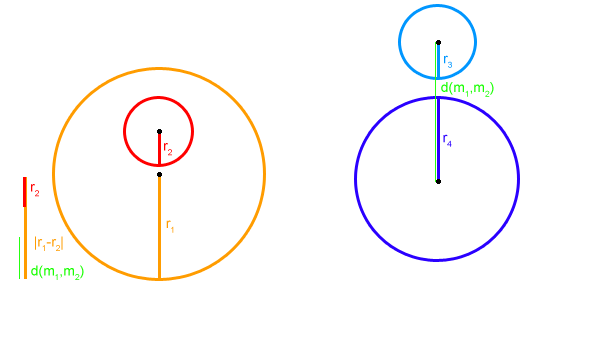
\includegraphics[scale=0.9]{2cirkels.png}
\caption{Niet snijdende cirkels}
\label{fig1}
\end{figure}

\newpage

\subsection*{1.2 Algoritme 2}

\begin{algorithm}
\caption{Bereken alle snijpunten van een verzameling cirkels met gebruik van een doorlooplijn}
\begin{algorithmic}
	\STATE \textbf{Input:} $cirkels$: Een lijst met $n$ cirkels
	\STATE $snijpunten$ $\gets$ $\emptyset$
	\STATE $actief$ $\gets \emptyset$ (Een verzameling die de  actieve cirkels bevat)
	\STATE $evenementen$: Een lijst die zowel de $x$-co\"ordinaat van het uiterste linkse als de $x$-co\"ordinaat van het uiterste rechtse punt van elke cirkel bevat, gesorteerd op de $x$-waarde.
    \FOR{each $evenement$ in $evenementen$}
       \IF{$evenement$ is $x$-co\"ordinaat van linkerpunt $cirkel$}
        \FOR{each $actieveCirkel$ in $actief$}
         \STATE voegToe($snijpunten$, berekenSnijpunten($cirkel$, $actieveCirkel$))
          \ENDFOR
         \STATE voegToe($actief$, $cirkel$)
         \ELSIF{$evenement$ is $x$-co\"ordinaat van rechterpunt $cirkel$}
         \STATE verwijder($actief$, $cirkel$)
         
        \ENDIF
    \ENDFOR
    \RETURN snijpunten
\end{algorithmic}
\end{algorithm}
De doorlooplijn zal van links naar rechts het gebied van cirkels doorlopen. Wanneer de doorlooplijn op een cirkel komt, zal deze vergeleken worden met de andere actieve cirkels om snijpunten te zoeken. Vervolgens wordt deze ook toegevoegd aan de verzameling van actieve cirkels. Wanneer de doorlooplijn een cirkel helemaal heeft doorlopen, zal deze cirkel verwijderd worden uit de verzameling van actieve cirkels.

We gaan de doorlooplijn natuurlijk enkel laten stoppen op linker- of rechterpunten van de cirkels. Dit kunnen we bereiken door vooraf een lijst op te stellen met ``evenementen'', die linker- en rechterpunten van cirkels voorstellen en gesorteerd is op de $x$-co\"ordinaten.

\newpage

\subsection*{1.3 Algoritme 3}

\begin{algorithm}
\caption{Bereken alle snijpunten van een verzameling cirkels met gebruik van een doorlooplijn, waarbij de actieve cirkels in een gesorteerde zoekboom geplaatst worden}
\begin{algorithmic}
	\STATE \textbf{Input:} $cirkels$: Een lijst met $n$ cirkels
	\STATE $snijpunten$ $\gets$ $\emptyset$
	\STATE $stralen \gets \emptyset$ (Een gesorteerde lijst met stralen van actieve cirkels)
	\STATE $actief$ $\gets \emptyset$ (Een zoekboom die de  actieve cirkels bevat, gesorteerd op de $y$-co\"ordinaat van hun middelpunt)
	\STATE $evenementen$: Een lijst die zowel de $x$-co\"ordinaat van het uiterste linkse als de $x$-co\"ordinaat van het uiterste rechtse punt van elke cirkel bevat, gesorteerd op de $x$-waarde.
	\STATE $maxStraal \gets$ 0 (Deze variabele houdt de straal van de grootste cirkel van de actieve cirkels bij).
    \FOR{each $evenement$ in $evenementen$}
       \IF{$evenement$ is $x$-co\"ordinaat van linkerpunt $cirkel$}
        \FOR{each $actieveCirkel$ in deelverzameling($actief$, $cirkel$.top.$y$ - $maxStraal$, $cirkel$.bottom.$y$ + $maxStraal$)}
			\IF{$actieveCirkel$.bottom.$y$ $\geq$ $cirkel$.top.$y$ en $actieveCirkel$.top.$y$ $\leq cirkel$.bottom.$y$}        
         \STATE voegToe($snijpunten$, berekenSnijpunten($cirkel$, $actieveCirkel$))
          \ENDIF
          \ENDFOR
         \IF{$cirkel$.straal groter dan $maxStraal$}
        	\STATE $maxStraal \gets cirkel$.straal
        \ENDIF
         \STATE voegToe($actief$, $cirkel$)
         \STATE voegToe($stralen$, $cirkel$.straal)
         \ELSIF{$evenement$ is $x$-co\"ordinaat van rechterpunt $cirkel$}
         \STATE verwijder($actief$, $cirkel$)
         \STATE verwijder($stralen$, $cirkel$.straal)
         \IF{$cirkel$.straal is $maxStraal$}
         	\STATE $maxStraal \gets pollFirst(stralen)$
        \ENDIF
        \ENDIF
    \ENDFOR
    \RETURN snijpunten
\end{algorithmic}
\end{algorithm}

De doorlooplijn zal werken zoals in \emph{Algoritme 2}. Nu vergelijken we de nieuwe actieve cirkel echter niet met elke andere actieve cirkel om snijpunten te berekenen. Dit doen we door een zoekboom te gebruiken waarin we de actieve cirkels plaatsen, gesorteerd op de $y$-co\"ordinaat van hun middelpunt. Verder gebruiken we ook een zoekboom waarin we de stralen van deze actieve cirkels zetten. Wanneer een nieuwe cirkel toegevoegd wordt, nemen we echter slechts een deelverzameling van de actieve cirkels. Deze deelverzameling bevat de cirkels waarvan het middelpunt minder ver ligt van het top- of het benedenpunt van de nieuwe actieve cirkel verlengd met de maximale straal. Van deze deelverzameling bekijken we enkel de cirkels waarvan een deel (van hun $y$-co\"ordinaten) tussen de nieuwe actieve cirkel ligt. De maximale straal zal indien nodig aangepast worden bij het toevoegen of verwijderen van een cirkel uit de verzameling van actieve cirkels.

\newpage
\section*{2. Experimenten}

We hebben de experimenten uitgevoerd door grafieken te maken van de uitvoeringstijd ten op zichte van het aantal cirkels. De grafieken werden opgesteld door willekeurige cirkels te genereren met een meegegeven maximum straal. We namen de gemiddelde uitvoertijd over 10 tests van deze gegenereerde cirkels. Eerst stelden we de maximale straal in op 0.01 en vervolgens verhoogden we deze systematisch. Hierdoor konden we de evolutie van de algoritmen evalueren voor verschillende stralen. Het aantal keer dat de methode ``berekenSnijpunten'' werd opgeroepen, werd ook gemeten, alsook het aantal snijpunten.

\subsection*{2.1 Relatief kleine stralen}
\begin{figure}[h]
\includegraphics[scale=0.5]{timebenchmark/{new_timeBenchmark0.01}.png}
\includegraphics[scale=0.5]{timebenchmark/{new_timeBenchmark0.1}.png}
\caption{Uitvoeringstijd van algoritme 1, 2 en 3 bij kleine stralen}
\label{tijdkleinestralen}
\end{figure}

In Figuur \ref{tijdkleinestralen} kunnen we zien dat \emph{Algoritme 1} duidelijk het slechtst presteert. Dit komt omdat het algoritme snijpunten zoekt door elke cirkel te vergelijken met elke andere cirkel. Hierdoor heeft het algoritme een tijdscomplexiteit van $O(n^2)$, aangezien het altijd $\frac{n(n-1)}{2}$ vergelijkingen uitvoert.\\

\emph{Algoritme 2} heeft een `slechtste-geval' rekencomplexiteit $O(n^2)$. In dit geval zijn de stralen echter zeer klein waardoor het veel beter presteert. Dit is te wijten aan het feit dat er weinig cirkels tegelijk actief zijn en er dus weinig cirkels vergeleken worden wanneer een nieuwe cirkel wordt toegevoegd. Figuur \ref{tijdkleinestralen} laat zien dat \emph{Algoritme 2} inderdaad veel beter presteert dan \emph{Algoritme 1} voor kleine stralen.\\

\emph{Algoritme 3} presteert beter met kleine stralen dan \emph{Algoritme 2} aangezien dit algoritme ook rekening houdt met de $y$-co\"ordinaten van de cirkels. De rekencomplexiteit is $O((n+S)log_2(n))$, waarbij $n$ het aantal cirkels is en $S$ het aantal snijpunten. Bij grotere stralen zal dit algoritme dus vertragen omdat er dan gemiddeld gesproken meer overlappende cirkels en dus ook meer snijpunten zijn.

\newpage

\begin{figure}[h]
\includegraphics[scale=0.5]{countbenchmarks/{new_countBenchmark0.01}.png}
\includegraphics[scale=0.5]{countbenchmarks/{new_countBenchmark0.1}.png}
\caption{Aantal keer dat ``berekenSnijpunten'' wordt opgeroepen door algoritme 1, 2 en 3 bij kleine stralen}
\label{countkleinestralen}
\end{figure}

Er is een discrepantie tussen het aantal keer dat de ``berekenSnijpunten'' methode wordt opgeroepen en de uitvoertijd. Dit is te wijten aan de complexe (gesorteerde) datastructuren die nodig zijn voor \emph{Algoritme 2} en \emph{3}. Dit is te zien in Figuur \ref{countkleinestralen}.\\

Zoals eerder vermeld, kunnen we in Figuur \ref{intersectkleinestralen} zien dat het aantal snijpunten zeer snel stijgt voor \'e\'enzelfde aantal cirkels indien de straal groter wordt. We zijn erin geslaagd om het aantal snijpunten zeer goed te benaderen alvorens het algoritme uitgevoerd wordt. Dit heeft als gevolg dat we de gegevensstructuur die gebruikt wordt om de snijpunten in op te slagen, een betere initi\"ele capaciteit kunnen meegegeven. Om het verwachte aantal snijpunten te berekenen, berekenen we de oppervlakte waarin een gemiddelde cirkel een andere cirkel snijdt. Een gemiddelde cirkel is bij onze gegenereerde cirkels een cirkel met een straal gelijk aan de maximale straal gedeeld door twee. Vervolgens nemen we de verhouding tussen deze oppervlakte en de totale oppervlakte van het vlak. Dit geeft de kans dat twee cirkels snijden. Om deze te extrapoleren naar de kans dat $n$ cirkels snijden, vermenigvuldigen we met $\frac{n(n-1)}{2}$. Hierna vermenigvuldigen we met twee omdat twee snijdende cirkels bijna altijd twee keer snijden.

\begin{center}
$gemiddeldeStraal = maxStraal/2$\\
$snijdingsOppervlakteGemiddeldeCirkel = \pi \times (2 \times gemiddeldeStraal)^2$\\
$verwachteAantalSnijpunten = \frac{snijdingsOppervlakteGemiddeldeCirkel}{totaleOppervlakte} * \frac{aantalCirkels \times (aantalCirkels-1)}{2} \times 2$
\end{center}

\begin{figure}[!h]
\includegraphics[scale=0.5]{intersectbenchmarks/{new_intersectBenchmark0.01}.png}
\includegraphics[scale=0.5]{intersectbenchmarks/{new_intersectBenchmark0.1}.png}
\caption{Schatting van aantal snijpunten samen met het werkelijk aantal snijpunten}
\label{intersectkleinestralen}
\end{figure}



\newpage
\subsection*{2.2 Relatief grote stralen}
\begin{figure}[!h]
\includegraphics[scale=0.5]{timebenchmark/{new_timeBenchmark0.2}.png}
\includegraphics[scale=0.5]{timebenchmark/{new_timeBenchmark0.5}.png}
\caption{Uitvoeringstijd van algoritme 1, 2 en 3 bij grote stralen}
\label{tijdgrotestralen}
\end{figure}
Grote stralen hebben geen invloed op het aantal vergelijkingen dat \emph{Algoritme 1} moet doen om te kijken of cirkels snijden. Zoals blijkt uit Figuur \ref{tijdgrotestralen} is er echter wel een verschil in uitvoeringstijd. Dit komt doordat het checken of twee cirkels snijden sneller is dan het daadwerkelijk berekenen van de snijpunten. Bij grote stralen zijn er veel meer snijpunten (zoals te zien is wanneer we Figuur \ref{intersectkleinestralen} en \ref{intersectgrotestralen} vergelijken), waardoor er meer snijpunten berekend zullen moeten worden.

\newpage
\begin{figure}[!h]
\includegraphics[scale=0.5]{countbenchmarks/{new_countBenchmark0.2}.png}
\includegraphics[scale=0.5]{countbenchmarks/{new_countBenchmark0.5}.png}
\caption{Aantal keer dat ``berekenSnijpunten'' wordt opgeroepen door \emph{Algoritme 1}, \emph{2} en \emph{3} bij grote stralen}
\label{countgrotestralen}
\end{figure}
\emph{Algoritme 2} is duidelijk trager bij grote cirkels dan bij kleine cirkels. Dit komt doordat cirkels langer actief blijven als ze een grotere straal hebben en er dus meer cirkels tegelijk actief zullen zijn. In het slechtste geval zullen alle cirkels tegelijk actief zijn. Hierdoor zal \emph{Algoritme 2} dezelfde rekencomplexiteit krijgen als \emph{Algoritme 1}, aangezien elke cirkel met elke andere cirkel vergeleken zal worden.\\

Aangezien \emph{Algoritme 3} een rekencomplexiteit heeft van $O((n+S)log_2(n))$, zal dit algoritme vertragen wanneer het aantal snijpunten toeneemt (zoals te zien in Figuur \ref{tijdgrotestralen}). In het slechtste geval, wanneer elke cirkel elke andere cirkel twee keer snijdt, zijn er $n(n-1)$ snijpunten. Hierdoor wordt de rekencomplexiteit van dit algoritme opgeblazen tot $O((n^2)log_2(n))$, wat duidelijk slechter is dan de rekencomplexiteit van \emph{Algoritme 1}. Dit zal echter nooit voorkomen in een re\"ele situatie.
\begin{figure}[!h]
\includegraphics[scale=0.5]{intersectbenchmarks/{new_intersectBenchmark0.2}.png}
\includegraphics[scale=0.5]{intersectbenchmarks/{new_intersectBenchmark0.5}.png}
\caption{Schatting van aantal snijpunten samen met het werkelijk aantal snijpunten}
\label{intersectgrotestralen}
\end{figure}
\newpage
\subsection*{2.3 Straal van maximum \'e\'en}
\begin{figure}[!h]
\includegraphics[scale=0.5]{timebenchmark/{new_timeBenchmark1.0}.png}
\includegraphics[scale=0.5]{countbenchmarks/{new_countBenchmark1}.png}
\caption{Uitvoeringstijd en aantal keer dat ``berekenSnijpunten'' wordt opgeroepen bij een straal van \'e\'en}
\label{straal1}
\end{figure}
Bij een straal van maximaal \'e\'en zien we dat hoewel het aantal vergelijken om snijpunten te berekenen bij \emph{Algoritme 3} nog steeds het laagst is, de uitvoeringstijd het hoogst is. Dit komt door de complexe gegevensstructuren die voor \emph{Algoritme 3} nodig zijn.

\section*{3. Het berekenen van snijpunten}
De methode die we gebruikt hebben om snijpunten te vinden, is gebaseerd op de methode die beschreven wordt in de volgende bron.

\subsection*{Bron}
N.N., How to calculate the intersection of two circles. Internet, 3 juli 2011, (http://fypandroid.wordpress.com/2011/07/03/how-to-calculate-the-intersection-of-two-circles-java/).

\end{document}